\documentclass[oneside]{book}
\usepackage{xcolor}
\usepackage{graphicx}
\usepackage{subcaption}

\graphicspath{{./picture/}}

\newcommand{\exercisename}{Latihan}
\newcommand{\solutionname}{Solusi}

\definecolor{main}{RGB}{0,120,2}

%% Exercise with counter
\newcounter{exer}[chapter]
\setcounter{exer}{0}
\renewcommand{\theexer}{\thechapter.\arabic{exer}}
\newenvironment{exercise}[1][]{
  \refstepcounter{exer}
  \par\noindent\textbf{\color{main}{\exercisename} \theexer #1 }\rmfamily}{
  \par\ignorespacesafterend}

\newenvironment{solution}{\par\noindent\textbf{\color{main}\solutionname} \em}{\par}

\begin{document}

\chapter{Digital Transmission}

% Johanes Wilian Ang 1-4
\begin{exercise}
  Contoh soal 1
\end{exercise}

\begin{solution}
  Contoh solusi
\end{solution}

\vspace{12pt}

\begin{exercise}
  Contoh soal
\end{exercise}

\begin{solution}
  Contoh solusi
\end{solution}

\vspace{12pt}

\begin{exercise}
  Contoh soal
\end{exercise}

\begin{solution}
  Contoh solusi
\end{solution}

\vspace{12pt}


\begin{exercise}
  Contoh soal
\end{exercise}

\begin{solution}
  Contoh solusi
\end{solution}

\vspace{12pt}

% Erwin Erikson 5-8
\begin{exercise}
  Contoh soal 5
\end{exercise}

\begin{solution}
  Contoh solusi
\end{solution}

\vspace{12pt}

\begin{exercise}
  Contoh soal
\end{exercise}

\begin{solution}
  Contoh solusi
\end{solution}

\vspace{12pt}

\begin{exercise}
  Contoh soal
\end{exercise}

\begin{solution}
  Contoh solusi
\end{solution}

\vspace{12pt}

\begin{exercise}
  Contoh soal
\end{exercise}

\begin{solution}
  Contoh solusi
\end{solution}

\vspace{12pt}

% Johnny 9-12
\begin{exercise}
  Contoh soal 9
\end{exercise}

\begin{solution}
  Contoh solusi
\end{solution}

\vspace{12pt}

\begin{exercise}
  Contoh soal
\end{exercise}

\begin{solution}
  Contoh solusi
\end{solution}

\vspace{12pt}

\begin{exercise}
  Contoh soal
\end{exercise}

\begin{solution}
  Contoh solusi
\end{solution}

\vspace{12pt}

\begin{exercise}
  Contoh soal
\end{exercise}

\begin{solution}
  Contoh solusi
\end{solution}

\vspace{12pt}

% Riani Artika 13-16
\begin{exercise}
  Contoh soal 13
\end{exercise}

\begin{solution}
  Contoh solusi
\end{solution}

\vspace{12pt}

\begin{exercise}
  Contoh soal
\end{exercise}

\begin{solution}
  Contoh solusi
\end{solution}

\vspace{12pt}

\begin{exercise}
  Contoh soal
\end{exercise}

\begin{solution}
  Contoh solusi
\end{solution}

\vspace{12pt}

\begin{exercise}
  Contoh soal
\end{exercise}

\begin{solution}
  Contoh solusi
\end{solution}

\vspace{12pt}

% Muhammad Al Imron 17-20
\begin{exercise}
  Contoh soal 17
\end{exercise}

\begin{solution}
  Contoh solusi
\end{solution}

\vspace{12pt}

\begin{exercise}
  Contoh soal
\end{exercise}

\begin{solution}
  Contoh solusi
\end{solution}

\vspace{12pt}

\begin{exercise}
  Contoh soal
\end{exercise}

\begin{solution}
  Contoh solusi
\end{solution}

\vspace{12pt}

\begin{exercise}
  Contoh soal
\end{exercise}

\begin{solution}
  Contoh solusi
\end{solution}

\chapter{Analog Transmission}

% Rian Sanjaya Nadeak 1-4
\begin{exercise}
  Calculate the baud rate for the given bit rate and type of modulation.
  \begin{itemize}
    \item[a.] 2000 bps, FSK
    \item[b.] 4000 bps, ASK
  \end{itemize}
\end{exercise}

\begin{solution}
  We use the formula $S = (1/r) \times N$, but first we need to calculate the value of r for each case.
  \begin{itemize}
    \item[a.] $r = log_22 = 1 \quad \rightarrow \quad S = (1/1) \times (2000 \textnormal{ bps}) = 2000 \textnormal{ baud}$
    \item[b.] 
  \end{itemize}
\end{solution}

\vspace{12pt}

\begin{exercise}
  Contoh soal
\end{exercise}

\begin{solution}
  Contoh solusi
\end{solution}

\vspace{12pt}

\begin{exercise}
  Contoh soal
\end{exercise}

\begin{solution}
  Contoh solusi
\end{solution}

\vspace{12pt}

\begin{exercise}
  Contoh soal
\end{exercise}

\begin{solution}
  Contoh solusi
\end{solution}

\vspace{12pt}

% R.m. Fikri Ihsan Kurniawan 5-8
\begin{exercise}
  Contoh soal 5
\end{exercise}

\begin{solution}
  Contoh solusi
\end{solution}

\vspace{12pt}

\begin{exercise}
  Contoh soal
\end{exercise}

\begin{solution}
  Contoh solusi
\end{solution}

\vspace{12pt}

\begin{exercise}
  Contoh soal
\end{exercise}

\begin{solution}
  Contoh solusi
\end{solution}

\vspace{12pt}

\begin{exercise}
  Contoh soal
\end{exercise}

\begin{solution}
  Contoh solusi
\end{solution}

\vspace{12pt}

% Farhan Ghulam Hadi Saputra 9-12
\begin{exercise}
  Contoh soal 9
\end{exercise}

\begin{solution}
  Contoh solusi
\end{solution}

\vspace{12pt}

\begin{exercise}
  Contoh soal
\end{exercise}

\begin{solution}
  Contoh solusi
\end{solution}

\vspace{12pt}

\begin{exercise}
  Contoh soal
\end{exercise}

\begin{solution}
  Contoh solusi
\end{solution}

\vspace{12pt}

\begin{exercise}
  Contoh soal
\end{exercise}

\begin{solution}
  Contoh solusi
\end{solution}

\chapter{Bandwidth Utilization: Multiplexing and Spreading}

% Hani Khairiyah 1-4
\begin{exercise}
  Contoh soal 1
\end{exercise}

\begin{solution}
  Contoh solusi
\end{solution}

\vspace{12pt}

\begin{exercise}
  Contoh soal
\end{exercise}

\begin{solution}
  Contoh solusi
\end{solution}

\vspace{12pt}

\begin{exercise}
  Contoh soal
\end{exercise}

\begin{solution}
  Contoh solusi
\end{solution}

\vspace{12pt}

\begin{exercise}
  Contoh soal
\end{exercise}

\begin{solution}
  Contoh solusi
\end{solution}

\vspace{12pt}

% Kevin Antony Kasamilale 5-8
\begin{exercise}
  Contoh soal 5
\end{exercise}

\begin{solution}
  Contoh solusi
\end{solution}

\vspace{12pt}

\begin{exercise}
  Contoh soal 6
\end{exercise}

\begin{solution}
  Contoh solusi
\end{solution}

\vspace{12pt}

\begin{exercise}
  Contoh soal
\end{exercise}

\begin{solution}
  Contoh solusi
\end{solution}

\vspace{12pt}

\begin{exercise}
  Contoh soal
\end{exercise}

\begin{solution}
  Contoh solusi
\end{solution}

\vspace{12pt}

% Annisa Wijaya 9-11
\begin{exercise}
  Contoh soal 9
\end{exercise}

\begin{solution}
  Contoh solusi
\end{solution}

\vspace{12pt}

\begin{exercise}
  Contoh soal
\end{exercise}

\begin{solution}
  Contoh solusi
\end{solution}

\vspace{12pt}

\begin{exercise}
  Contoh soal
\end{exercise}

\begin{solution}
  Contoh solusi
\end{solution}

\vspace{12pt}

% Andrian Syah 12-14 test push ke github
\begin{exercise}
  Contoh soal 12 : Gambar dibawah ini menunjukkan multiplexer dalam sistem TDM sinkron. Setiap slot keluaran adalah
  panjangnya hanya 10 bit (3 bit diambil dari setiap input ditambah 1 bit framing). Apa keluarannya?
  jalur kecil? Bit tiba di multiplexer seperti yang ditunjukkan oleh panah.
\end{exercise}

\begin{figure}[h]
  \centering
  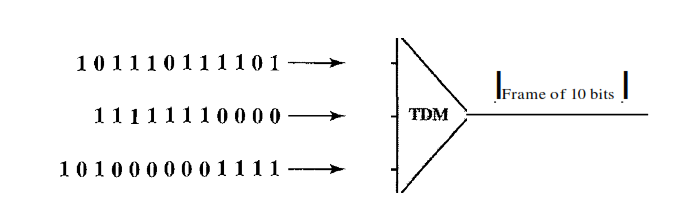
\includegraphics[width=0.9\textwidth]{soal12.png}
\end{figure}

\begin{solution}

\end{solution}

\begin{figure}[h]
  \centering
  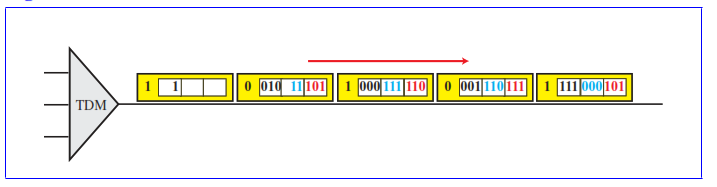
\includegraphics[width=0.9\textwidth]{solusi12.png}
\end{figure}

\vspace{12pt}

\begin{exercise}
  Contoh soal 13 : Gambar 3.1 dibawah menunjukkan demultiplexer dalam TDM sinkron. Jika slot input adalah 16 bit
  panjang (tanpa bit framing), apa aliran bit di setiap output? Bit tiba di
  demultiplexer seperti yang ditunjukkan oleh panah.

  \begin{figure}[h]
    \centering
    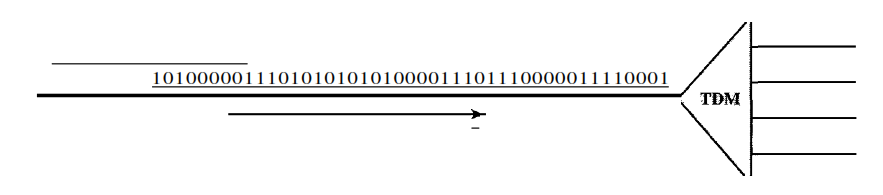
\includegraphics[width=0.9\textwidth]{soal13.png}
    \caption{TDM}
  \end{figure}

\end{exercise}


\vspace{40pt}

\begin{solution}
  \begin{figure}[h]
    \centering
    
\includegraphics[width=0.9\textwidth]{solusi13.png}
    \caption{solusi TDM}
  \end{figure}
\end{solution}




\begin{exercise}
  Jawab pertanyaan berikut tentang hierarki digital pada Gambar 3.3:
  \begin{itemize}
    \item[a.] Berapa overhead (jumlah bit tambahan) dalam layanan DS-l?
    \item[b.] Berapa overhead (jumlah bit tambahan) dalam layanan DS-2?
    \item[c.] Berapa overhead (jumlah bit tambahan) dalam layanan DS-3?
    \item[d.] Berapa overhead (jumlah bit tambahan) dalam layanan DS-4?
  \end{itemize}
\end{exercise}

\begin{figure}[h]
  \centering
  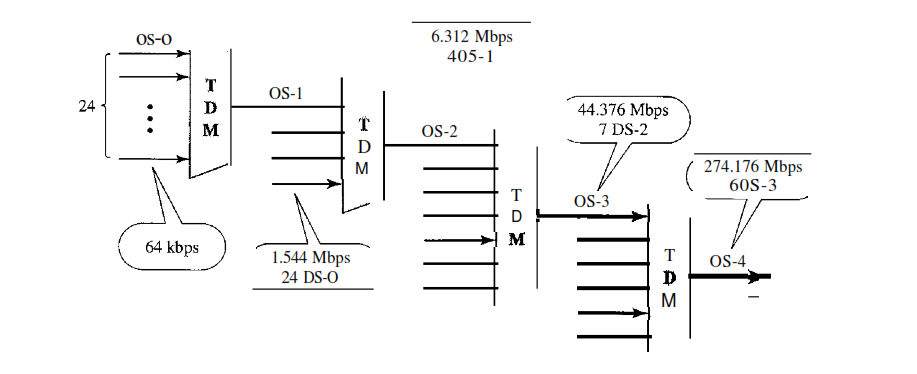
\includegraphics[width=0.9\textwidth]{figure6.23.png}
  \caption{Hierarki Digital}
\end{figure}

\begin{solution}
  \begin{itemize}
    \item[a.] DS-1 Overhead = 
    \begin{math}
       1.544 Mbps - (24 \times 64 kbps) = 8 kbps 
    \end{math}
   \item [b.] DS-2 Overhead =
        \begin{math}
          6.312 Mbps - (4 \times 1.544 kbps) = 136 kbps 
        \end{math}
   \item [c.] DS-3 Overhead =
        \begin{math}
          44.376 Mbps - (7 \times 6.312 kbps) = 192 kbps 
        \end{math}
   \item [d.] DS-4 Overhead =
   \begin{math}
    274.176 Mbps - (6 \times 44.376 kbps) = 7.92 Mbps 
  \end{math}
  \end{itemize}
\end{solution}

\vspace{12pt}

% Maranti Nainggolan 15-18
\begin{exercise}
  Contoh soal 15
\end{exercise}

\begin{solution}
  Contoh solusi
\end{solution}

\vspace{12pt}

\begin{exercise}
  Contoh soal 16
\end{exercise}

\begin{solution}
  Contoh solusi
\end{solution}

\vspace{12pt}

\begin{exercise}
  Contoh soal 17
\end{exercise}

\begin{solution}
  Contoh solusi
\end{solution}

\vspace{12pt}

\begin{exercise}
  Contoh soal
\end{exercise}

\begin{solution}
  Contoh solusi
\end{solution}

\end{document}

